\documentclass[a4paper,10.5pt]{article}

% ---- Page layout ----
\usepackage[margin=2.2cm]{geometry}
\setlength{\parindent}{0pt}
\setlength{\parskip}{0.5em}

% ---- Fonts (XeLaTeX; needed for correct Vietnamese diacritics) ----
\usepackage{fontspec}

% ---- Typography & links ----
\usepackage{microtype}
\usepackage{xcolor}
\usepackage{hyperref}
\hypersetup{colorlinks = true, linkcolor = blue!50!black, urlcolor = blue!50!black}

% ---- Figures & tables ----
\usepackage{graphicx}
\usepackage{booktabs}
\usepackage{array}

% ---- Header / footer ----
\usepackage{fancyhdr}
\pagestyle{fancy}
\fancyhf{}
\rfoot{\thepage}
\renewcommand{\headrulewidth}{0pt}

\begin{document}

\begin{center}
    {\LARGE\bfseries Customer Retention \& Churn Prediction}\\[0.2cm]
    {\large Executive Brief}\\[0.15cm]
    {\small Business Data Analytics Project Report \textbar{} \today}
\end{center}

\vspace{0.3cm}
\rule{\linewidth}{0.6pt}
\vspace{0.1cm}

\section{The Opportunity}
Retaining an existing customer costs far less than acquiring a new one, and revenue is highly concentrated: the \textbf{top 5\% of customers generate 52\% of revenue}, and the top 10\% generate 64\%. Protecting this base from churn is where retention spend has the most leverage.

\begin{center}
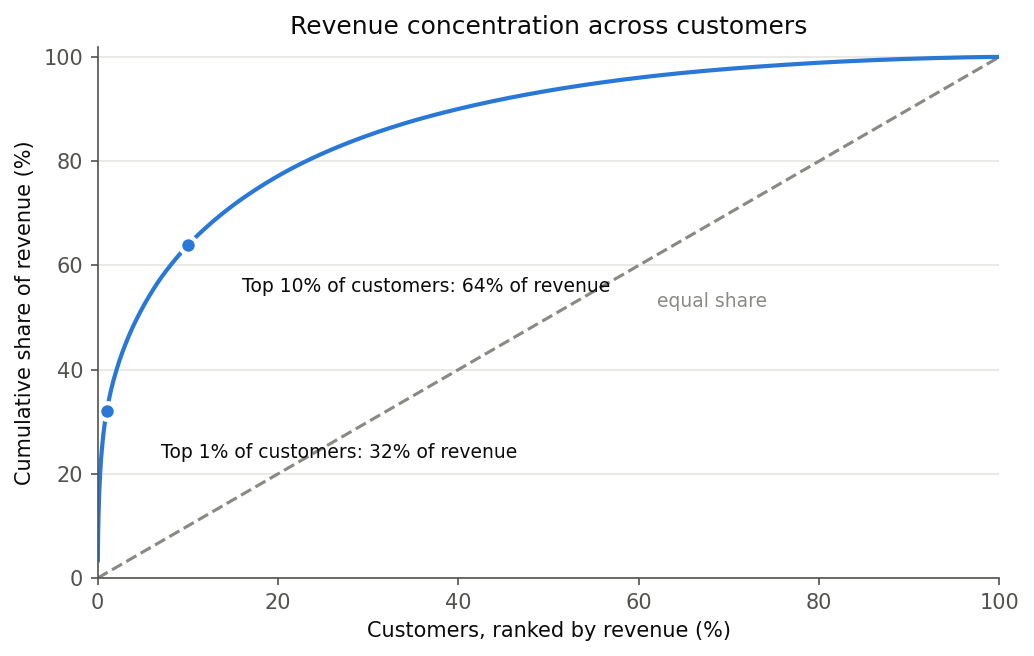
\includegraphics[width=0.48\textwidth]{figures/value_concentration.png}
\end{center}

\section{What We Built}
A weekly churn early-warning score for every active customer, built on point-in-time RFM and purchase-behavior features and a Logistic Regression classifier. On a held-out 10-week test period (2,907 customers, 40.1\% churned), the model reaches \textbf{ROC-AUC 0.765} and \textbf{PR-AUC 0.658} -- clearly separating customers likely to lapse within 90 days from those who will return, and leading every rule-based baseline on ranking quality (Precision@10\% $0.760\pm0.050$, Lift@10\% $1.902\pm0.055$) in every one of the 10 test weeks.

\section{Key Finding: Risk Is Not the Same as Value}
Despite leading every predictive and ranking metric, the model is \textbf{not} the most profitable targeting rule at the standard 10\% operating point. Comparing estimated net business impact of contacting the top 10\% of customers each week (40\% offer response rate, 35\% margin, \pounds0.50 contact cost, \pounds5.00 incentive cost):

\begin{center}
\begin{tabular}{@{}p{3.6cm}p{2.6cm}p{3.4cm}@{}}
    \toprule
    Targeting rule & Churners caught & Net business impact \\
    \midrule
    \textbf{Churn model} & \textbf{1,846} & \textbf{\pounds42,388} \\
    RFM score (hand-built) & 1,743 & \pounds64,345 \\
    Longest time since last purchase & 1,521 & \textbf{\pounds70,214} \\
    Random & 986 & \pounds41,626 \\
    \bottomrule
\end{tabular}
\end{center}

The model catches far more churners than the simple rules, yet ends up \emph{less} profitable. The reason: a customer's average order value is only weakly related to their churn risk (\pounds269 vs.\ \pounds324 median, churned vs.\ not) -- so ranking purely by churn probability does not automatically prioritize high-value customers. The simpler rules happen to catch a higher-value subset, even while catching fewer churners overall.

\section{Recommendation}
Before a wide rollout, change the targeting score from ``churn probability'' to \textbf{expected value} (probability $\times$ customer value), so retention spend is prioritized by both risk \emph{and} revenue -- not risk alone. Validate with a real pilot campaign against a held-out control group: this dataset contains no past campaign data, so every pound figure above is a scenario estimate under the stated assumptions, not an observed outcome.

\end{document}
